\chapter{Preparationskammer}

Das Wachstum wurde in einer Ultra-Hoch Vakuum (UHV) Kammer durchgeführt, die auf das Wachstum und die Analyse dünner Schichtsysteme ausgelegt ist.
Der Basisdruck in der Kammer liegt in der Größenordnung von $p=1\cdot 10^{-10}\,\si{\milli\bar}$.
Zur ständigen Druckmessung wird dabei ein Ionisations-Vakuummeter (ion gauge) verwendet.
In die Kammer können über leak Ventile $\symup{Ar}^+$-Ionen sowie $\symup{O_2}$-Moleküle 
eingelassen werden. 

Die $\symup{Ar}^+$-Ionen werden dabei zum Reinigen der Probe bei der Ioneninduzierten Zerstäubung (sputtering) verwendet.
Diese können durch eine angelegte Spannung unter einem Winkel auf die Probe beschleunigt werden und tragen durch Stöße Oberflächenatome ab.
Durch anschlißendes Heizen der Probe desorbieren weitere Verunreinigungen und durch die zusätzliche thermische Energie ordnet sich die 
Oberfläche neu.

Die Probe ist in der Kammer durch einen Manipulator frei translatierbar und außerdem um $360\,\si{\degree}$ um die z-Achse rotierbar.
Am Manipulator ist außerdem eine QCM befestigt, die in der Höhe und  Tiefe versetzt zur Probenhalterung angebracht ist.

Der MG-Aufdampfer steht im $90\,\si{\degree}$ Winkel zum LEED Schrim und zur Elektronenquelle des AES, was MEED Messungen während des Aufdampfens ermöglicht.
Für unterschiedliche Winkel zwischen Probe und LEED Schirm stellen sich verschiedene Beugungsordnungen ein, welche in Abbildung \ref{fig:MEED-Bilder} zu sehen sind.



\begin{figure}[H]
    \centering
    \subfloat[][]{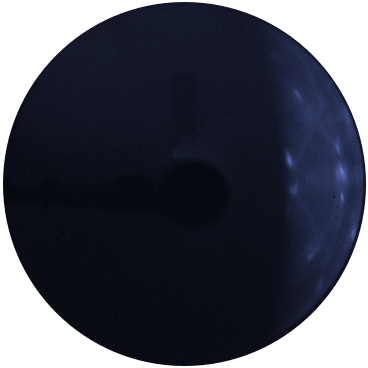
\includegraphics[width=0.28\linewidth]{Plots/MEED_103_degree.png}}%
    \qquad
    \subfloat[][]{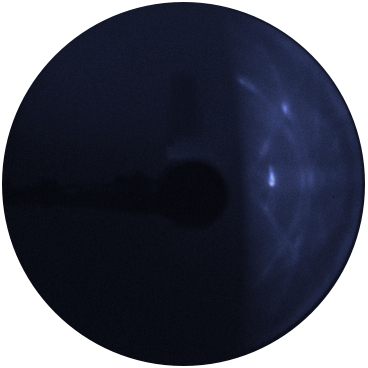
\includegraphics[width=0.28\linewidth]{Plots/MEED_109_degree.png}}%
    \qquad
    \subfloat[][]{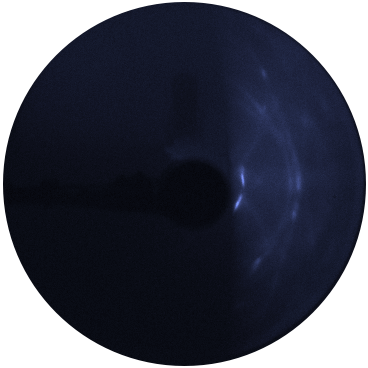
\includegraphics[width=0.28\linewidth]{Plots/MEED_113_degree.png}}%
    \caption{Bilder des LEED Schirms mit MEED Einstellungen für verschiedene Winkel zwischen Probe und Schirm. 
            (a) zeigt einen Winkel von $13\,\si{\degree}$, (b) einen Winkel von $7\,\si{\degree}$ und (c) einen Winkel von $3\,\si{\degree}$ zwischen Probe und Schirm.}%
    \label{fig:MEED-Bilder}
  \end{figure}

